\clearpage{\pagestyle{empty}\cleardoublepage}
\chapter{Introduzione del sistema}
\lhead[\fancyplain{}{\bfseries\thepage}]{\fancyplain{}{\bfseries\rightmark}}
\pagenumbering{arabic}

Il primo capitolo ha due obiettivi:
il primo obiettivo è l'introduzione del progetto di tesi, con le sue caratteristiche e funzionalità;
il secondo obiettivo è l'analisi dello stato dell'arte degli attuali sistemi simili al progetto dell'elaborato di tesi,
descrivendone le caratteristiche principali, ponendo i diversi sistemi a confronto e approfondendone le funzionalità.

\section{Scopo del progetto}

Lo scopo del progetto di tesi è quello di presentare un sistema di simulazione atto alla collezione ed interpretazione
di dati sulla qualità dell'aria di una determinata area geografica.

Tali dati provengono da misurazioni fittizie prodotte da sensori distribuiti in un'area di studio.
I sensori inviano delle rilevazioni ad un intermediario, il quale le raccoglie e rende disponibili.
Viene quindi disposta una dashboard attraverso la quale gli utenti possono fruirne sotto forma di tabelle e di una mappa interattiva.

La dashboard consiste in una web app mobile-first che permette di visualizzare l'area geografica coinvolta e
i dati sulla qualità dell'aria.
Lo sviluppo della dashboard prende come riferimento le applicazioni della stessa tipologia attualmente presenti
come stato dell'arte.

L'area geografica di interesse è il comune di Bologna, entro il cui perimetro vengono posizionati i sensori
di simulazione \cite{Accuweather}.

\section{Qualità dell'aria}
I dati sulla qualità dell'aria vengono definiti dai paesi secondo indici e scale.
L'indice di qualità dell'aria (IQA) rappresenta il modo in cui i governi scelgono di comunicare con la popolazione
la qualità dell'aria. Esso converge il livello di diversi inquinanti in un unico indice comprensibile,
consentendo di identificare più facilmente il livello di inquinamento e l'eventuale rischio associato.

Regioni e paesi diversi utilizzano scale differenti per indicare la qualità dell'aria in base all'inquinamento locale e
a considerazioni sulla salute. Esistono decine di indici locali utilizzati in tutto il mondo;
ad esempio, in alcune regioni dell'Australia si utilizzano sistemi basati su numeri, mentre altre ne usano uno basato
su categorie. Canada, Giappone e Stati Uniti definiscono indici di qualità dell'aria distinti, così come
l'Agenzia europea dell'ambiente \cite{EuropeanEnvironmentAgency}.

Il servizio online \href{https://airindex.eea.europa.eu/AQI/index.html}{"The European Air Quality Index" (EAQI)} dell'\href{https://www.eea.europa.eu/it}{EEA (European Environment Agency)} e
della \href{https://commission.europa.eu/index_it}{Commissione Europea} fornisce informazioni sulla qualità dell'aria basate su più di 2000 stazioni di rilevamento
in tutta Europa \cite{EEA2017IndiceEuropeo}. L'indice consiste in una mappa interattiva che mostra la qualità dell'aria a livello locale,
andando ad analizzare i 5 livelli di inquinanti più pericolosi per le persone e per l'ambiente:

\begin{itemize}
  \item Particolato PM2.5 e PM10
  \item Ozono (O3)
  \item Diossido di azoto (NO2)
  \item Anidride solforosa (SO2)
\end{itemize}

Gli utenti possono zoommare la mappa o ricercare città Europee per controllare la qualità globale dell'aria e verificare i livelli di inquinanti registrati dai sensori dalle stazioni locali. L'Indice mostra un rating globale per ogni stazione di rilevamento, andando a marcare la mappa con un punto colorato, per ognuno dei 5 inquinanti. Il colore indica un livello di qualità dell'aria:
\begin{itemize}
  \item Molto buono (verde acqua)
  \item Buono (verde)
  \item Moderato (giallo)
  \item Basso (rosso)
  \item Molto basso (rosso ciliegia)
  \item Estremamente basso (viola)
\end{itemize}

Nella tabella \ref{tab:air_quality} sono riportati i valori relativi al livello di qualità dell'aria.

\begin{table}[h]
  \centering
  \adjustbox{width=\textwidth,center}{
    \begin{tabular}{|>{\raggedright\arraybackslash}m{3cm}|c|c|c|c|c|c|}
      \hline
      \textbf{Inquinante}
       & \textbf{Buono}
       & \textbf{Discreto}
       & \textbf{Moderato}
       & \textbf{Scarso}
       & \textbf{Molto scarso}
       & \textbf{Estremamente scarso}               \\
      \hline
      Particelle inferiori a 2.5 $\mu$m (PM$_{2.5}$)
       & \cellcolor{good}0-5
       & \cellcolor{fair}\color{white}6-15
       & \cellcolor{moderate}16-50
       & \cellcolor{poor}\color{white}51-90
       & \cellcolor{verypoor}\color{white}91-140
       & \cellcolor{extremelypoor}\color{white}>140 \\
      \hline
      Particelle inferiori a 10 $\mu$m (PM$_{10}$)
       & \cellcolor{good}0-15
       & \cellcolor{fair}\color{white}16-45
       & \cellcolor{moderate}46-120
       & \cellcolor{poor}\color{white}121-195
       & \cellcolor{verypoor}\color{white}196-270
       & \cellcolor{extremelypoor}\color{white}>270 \\
      \hline
      Biossido di azoto (NO$_2$)
       & \cellcolor{good}0-60
       & \cellcolor{fair}\color{white}61-100
       & \cellcolor{moderate}101-120
       & \cellcolor{poor}\color{white}121-160
       & \cellcolor{verypoor}\color{white}161-180
       & \cellcolor{extremelypoor}\color{white}>180 \\
      \hline
      Ozono (O$_3$)
       & \cellcolor{good}0-10
       & \cellcolor{fair}\color{white}11-25
       & \cellcolor{moderate}26-60
       & \cellcolor{poor}\color{white}61-100
       & \cellcolor{verypoor}\color{white}101-150
       & \cellcolor{extremelypoor}\color{white}>150 \\
      \hline
      Biossido di zolfo (SO$_2$)
       & \cellcolor{good}0-20
       & \cellcolor{fair}\color{white}21-40
       & \cellcolor{moderate}41-125
       & \cellcolor{poor}\color{white}126-190
       & \cellcolor{verypoor}\color{white}191-275
       & \cellcolor{extremelypoor}\color{white}>275 \\
      \hline
    \end{tabular}
  }
  \caption{Indici di qualità dell'aria per diversi inquinanti secondo l'EAQI, concentrazioni espresse in $\mu g/m^3$
 \cite{EuropeanAirQualityMapAndCharts}.}
  \label{tab:air_quality}
\end{table}

% \begin{figure}
%   \centering
%   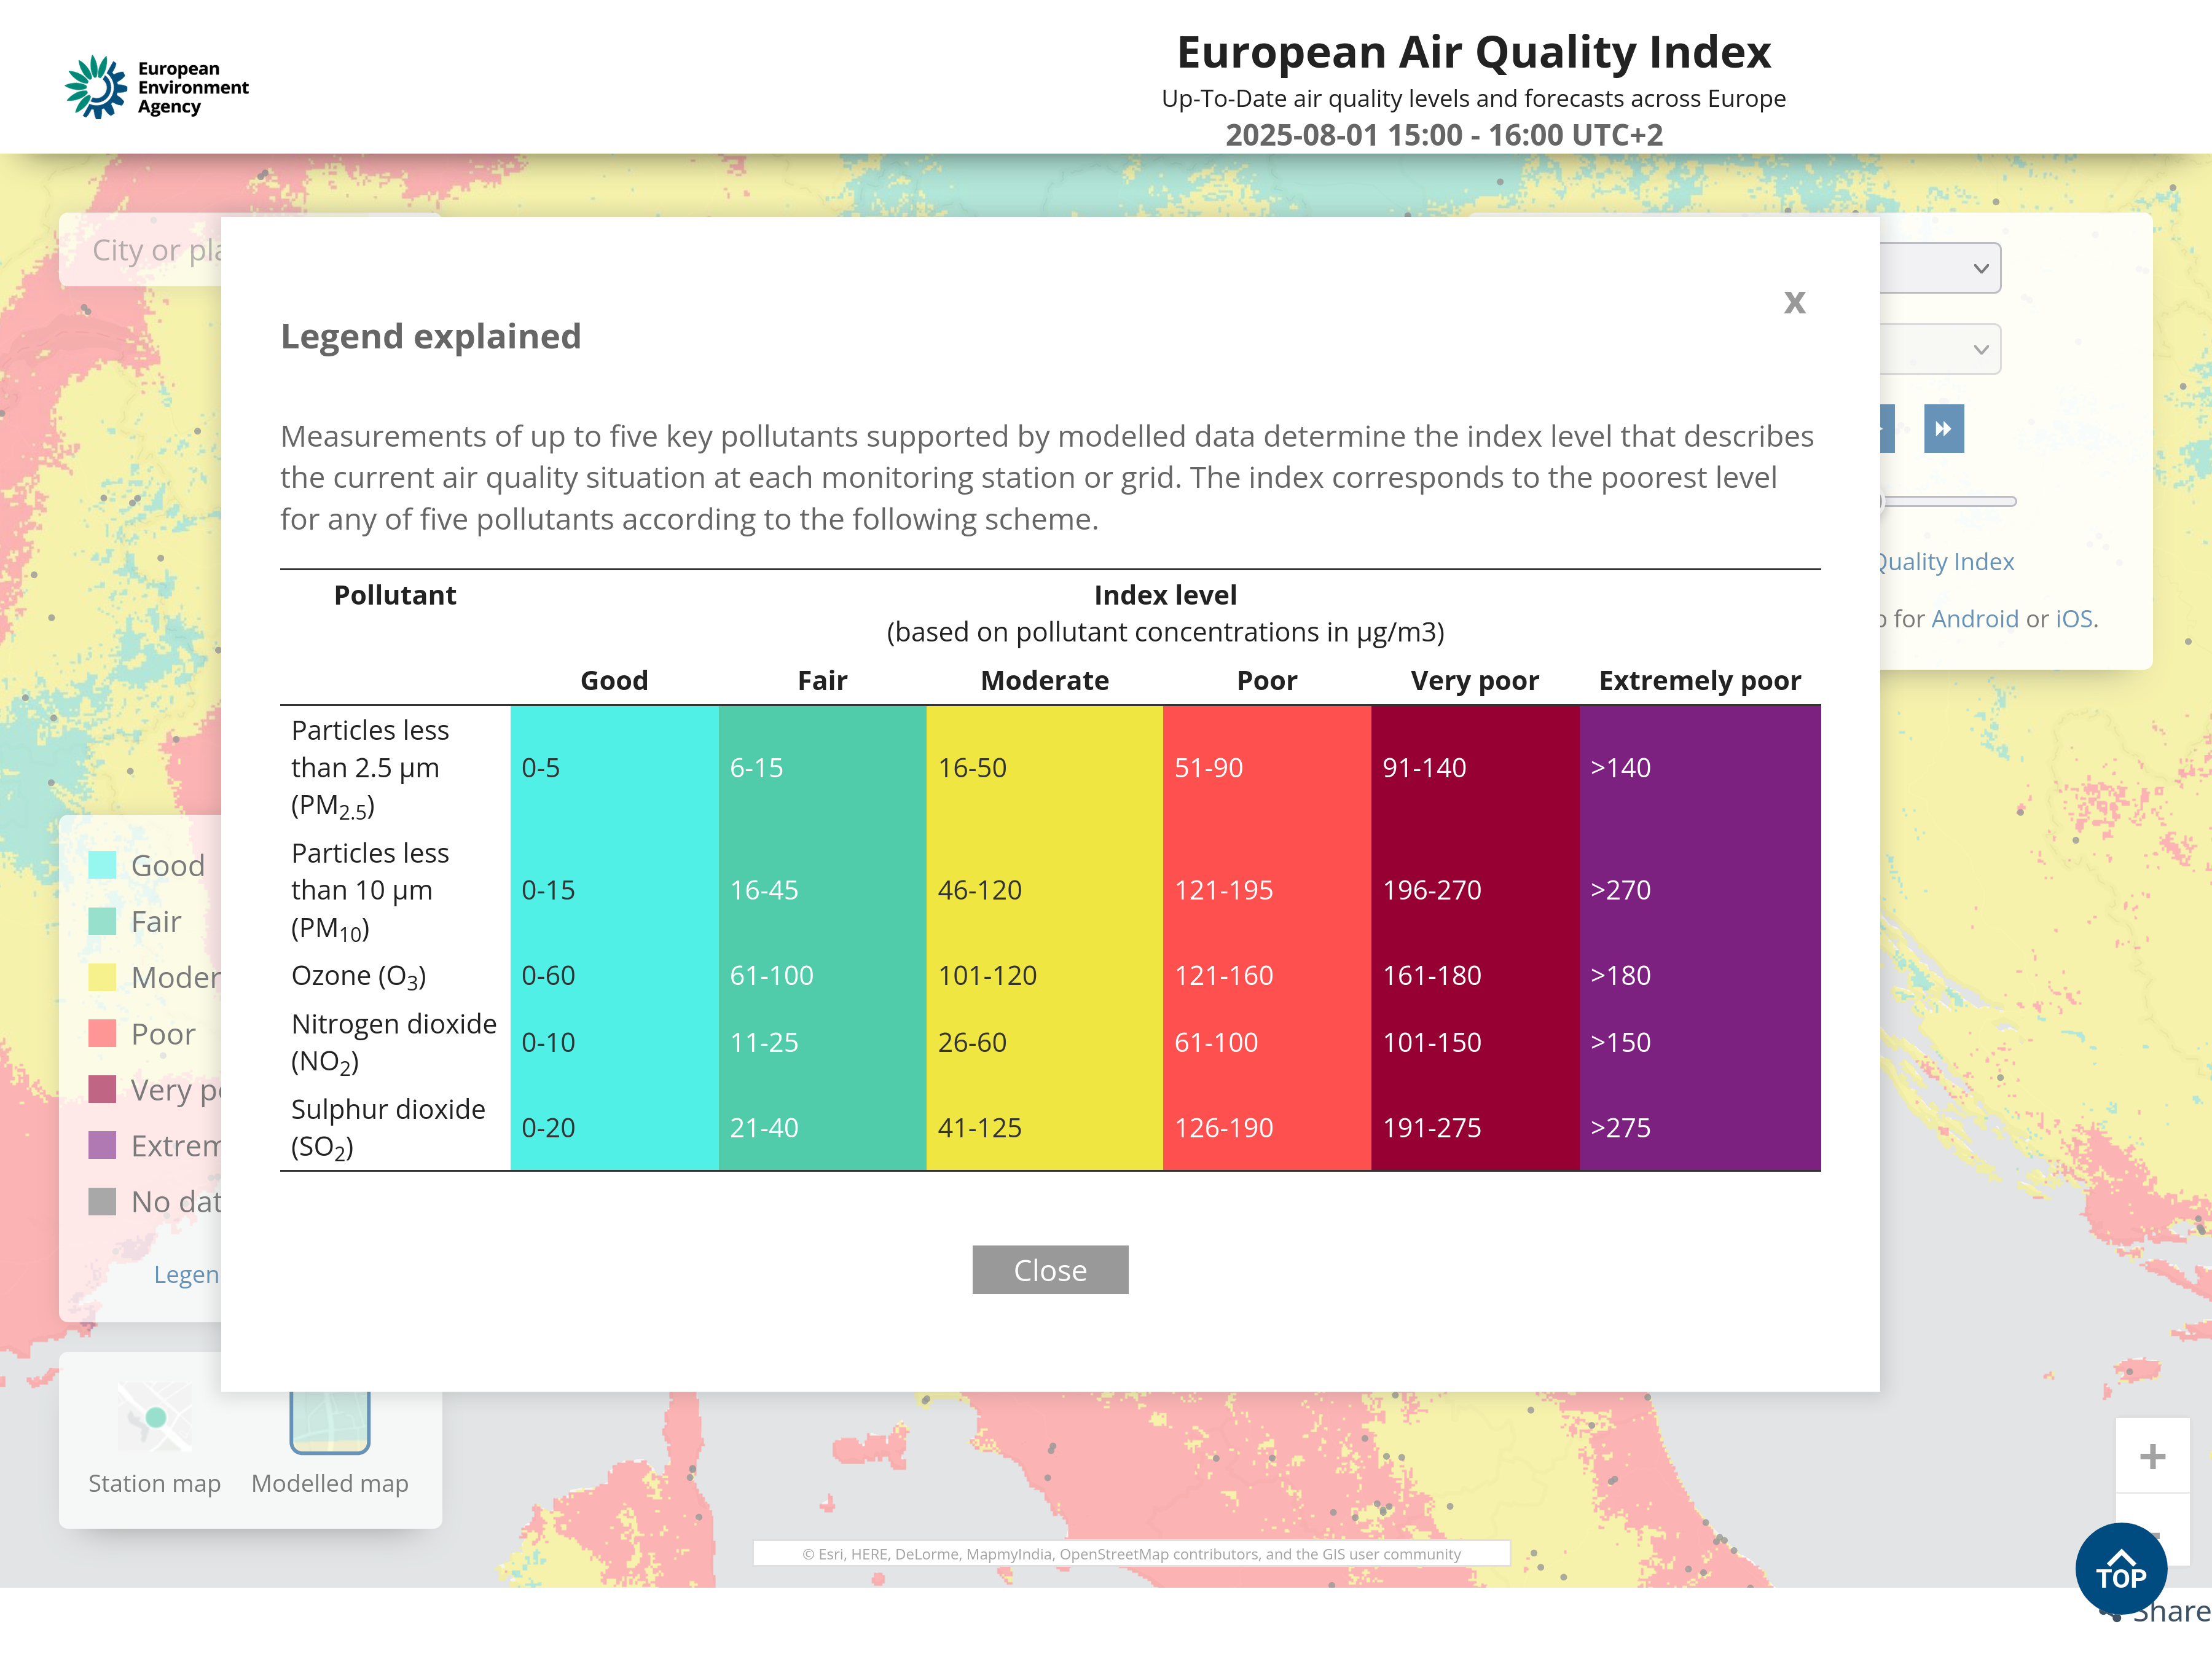
\includegraphics[width=\textwidth]{eea_4.png}
%   %\includegraphics[width=5cm]{figura.eps}%inserisce una figura larga 5cm
%   \caption[legenda elenco figure]{legenda sotto la figura}
%   \label{fig:prima}
% \end{figure}

\newpage

Il portale riporta inoltre una serie di messaggi atti a fornire raccomandazioni, sia alla fascia di popolazione normale che a quella più sensibile, in funzione dell'AQI misurato. La fascia di soggetti più sensibile comprende sia adulti che bambini con problemi respiratori che cardiaci. 

Nella tabella \ref{tab:health-messages} vengono indicati i messaggi suggeriti alle fasce di popolazione relative in relazione al livello di qualità dell'aria.

\begin{table}[H]
  \centering
  \adjustbox{width=\textwidth,center}{
    \begin{tabular}{|>{\centering\arraybackslash}m{3cm}|p{6cm}|p{6cm}|}
     \hline
      \textbf{AQI}
      & \textbf{Popolazione normale}
      & \textbf{Popolazione sensibile} \\
      \hline
      \cellcolor{good} Buono
      & La qualità dell'aria è buona.\newline Goditi le tue solite attività all'aperto.
      & La qualità dell'aria è buona.\newline Goditi le tue solite attività all'aperto.\\
      \hline
      \cellcolor{fair}\color{white} Discreto
      & Goditi le tue solite attività all'aperto.
      & Goditi le tue solite attività all'aperto.\\
      \hline
      \cellcolor{moderate} Moderato
      & Goditi le tue solite attività all'aperto.
      & Considera di ridurre le attività intense all'aperto, se avverti sintomi.\\
      \hline
      \cellcolor{poor}\color{white} Scadente
      & Considera di ridurre le attività intense all'aperto, se avverti sintomi come irritazione agli occhi, tosse o mal di gola.
      & Considera di ridurre le attività fisiche, soprattutto all'aperto, specialmente se avverti sintomi.\\
      \hline
      \cellcolor{verypoor}\color{white} Molto scadente
      & Considera di ridurre le attività intense all'aperto, se avverti sintomi come irritazione agli occhi, tosse o mal di gola.
      & Riduci le attività fisiche, soprattutto all'aperto, specialmente se avverti sintomi.\\
      \hline
      \cellcolor{extremelypoor}\color{white} Estremamente scadente
      & Riduci le attività fisiche all'aperto.
      & Evita le attività fisiche all'aperto.\\
    \end{tabular}
    }
  \caption{Messaggi relativi alla salute}
  \label{tab:health-messages}
\end{table}

Nelle seguenti figure \ref{fig:eaqi-combined} vengono mostrate le due possibili grafiche della mappa interattiva riportante l'European Air Quality Index (EAQI).

\begin{figure}[H]
  \centering
  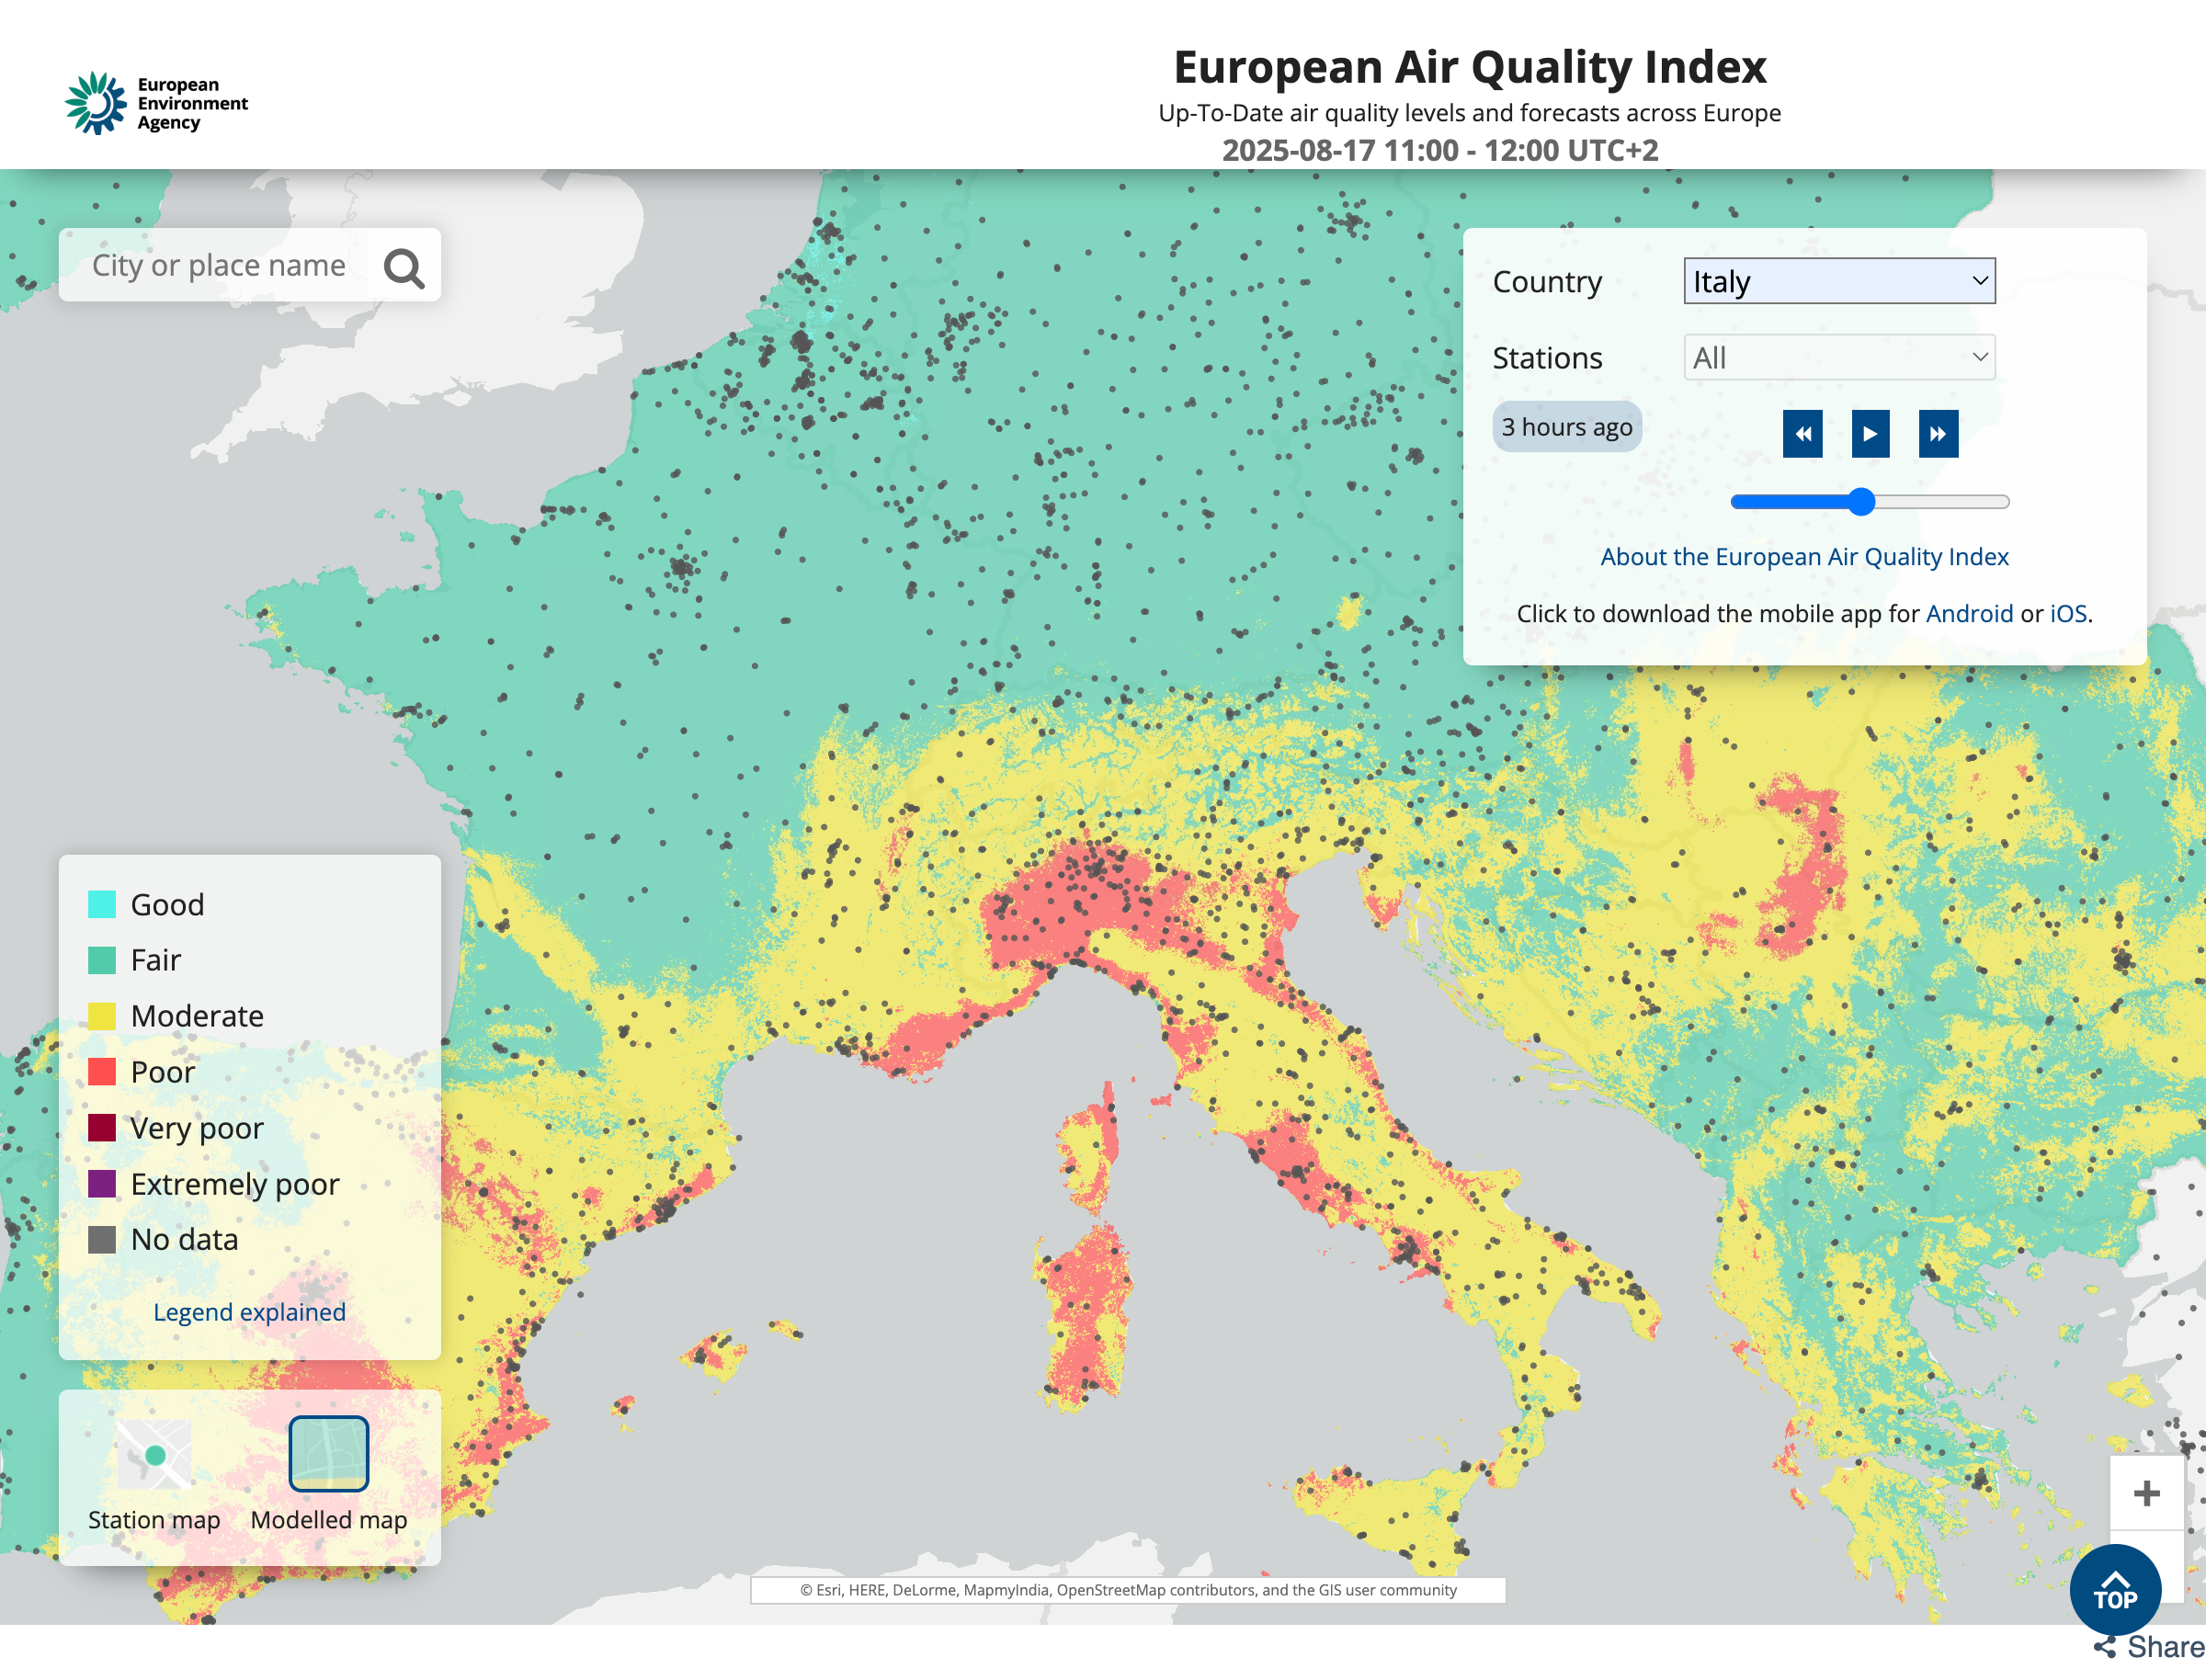
\includegraphics[width=\textwidth]{eaqi2.png}\\[1em]
  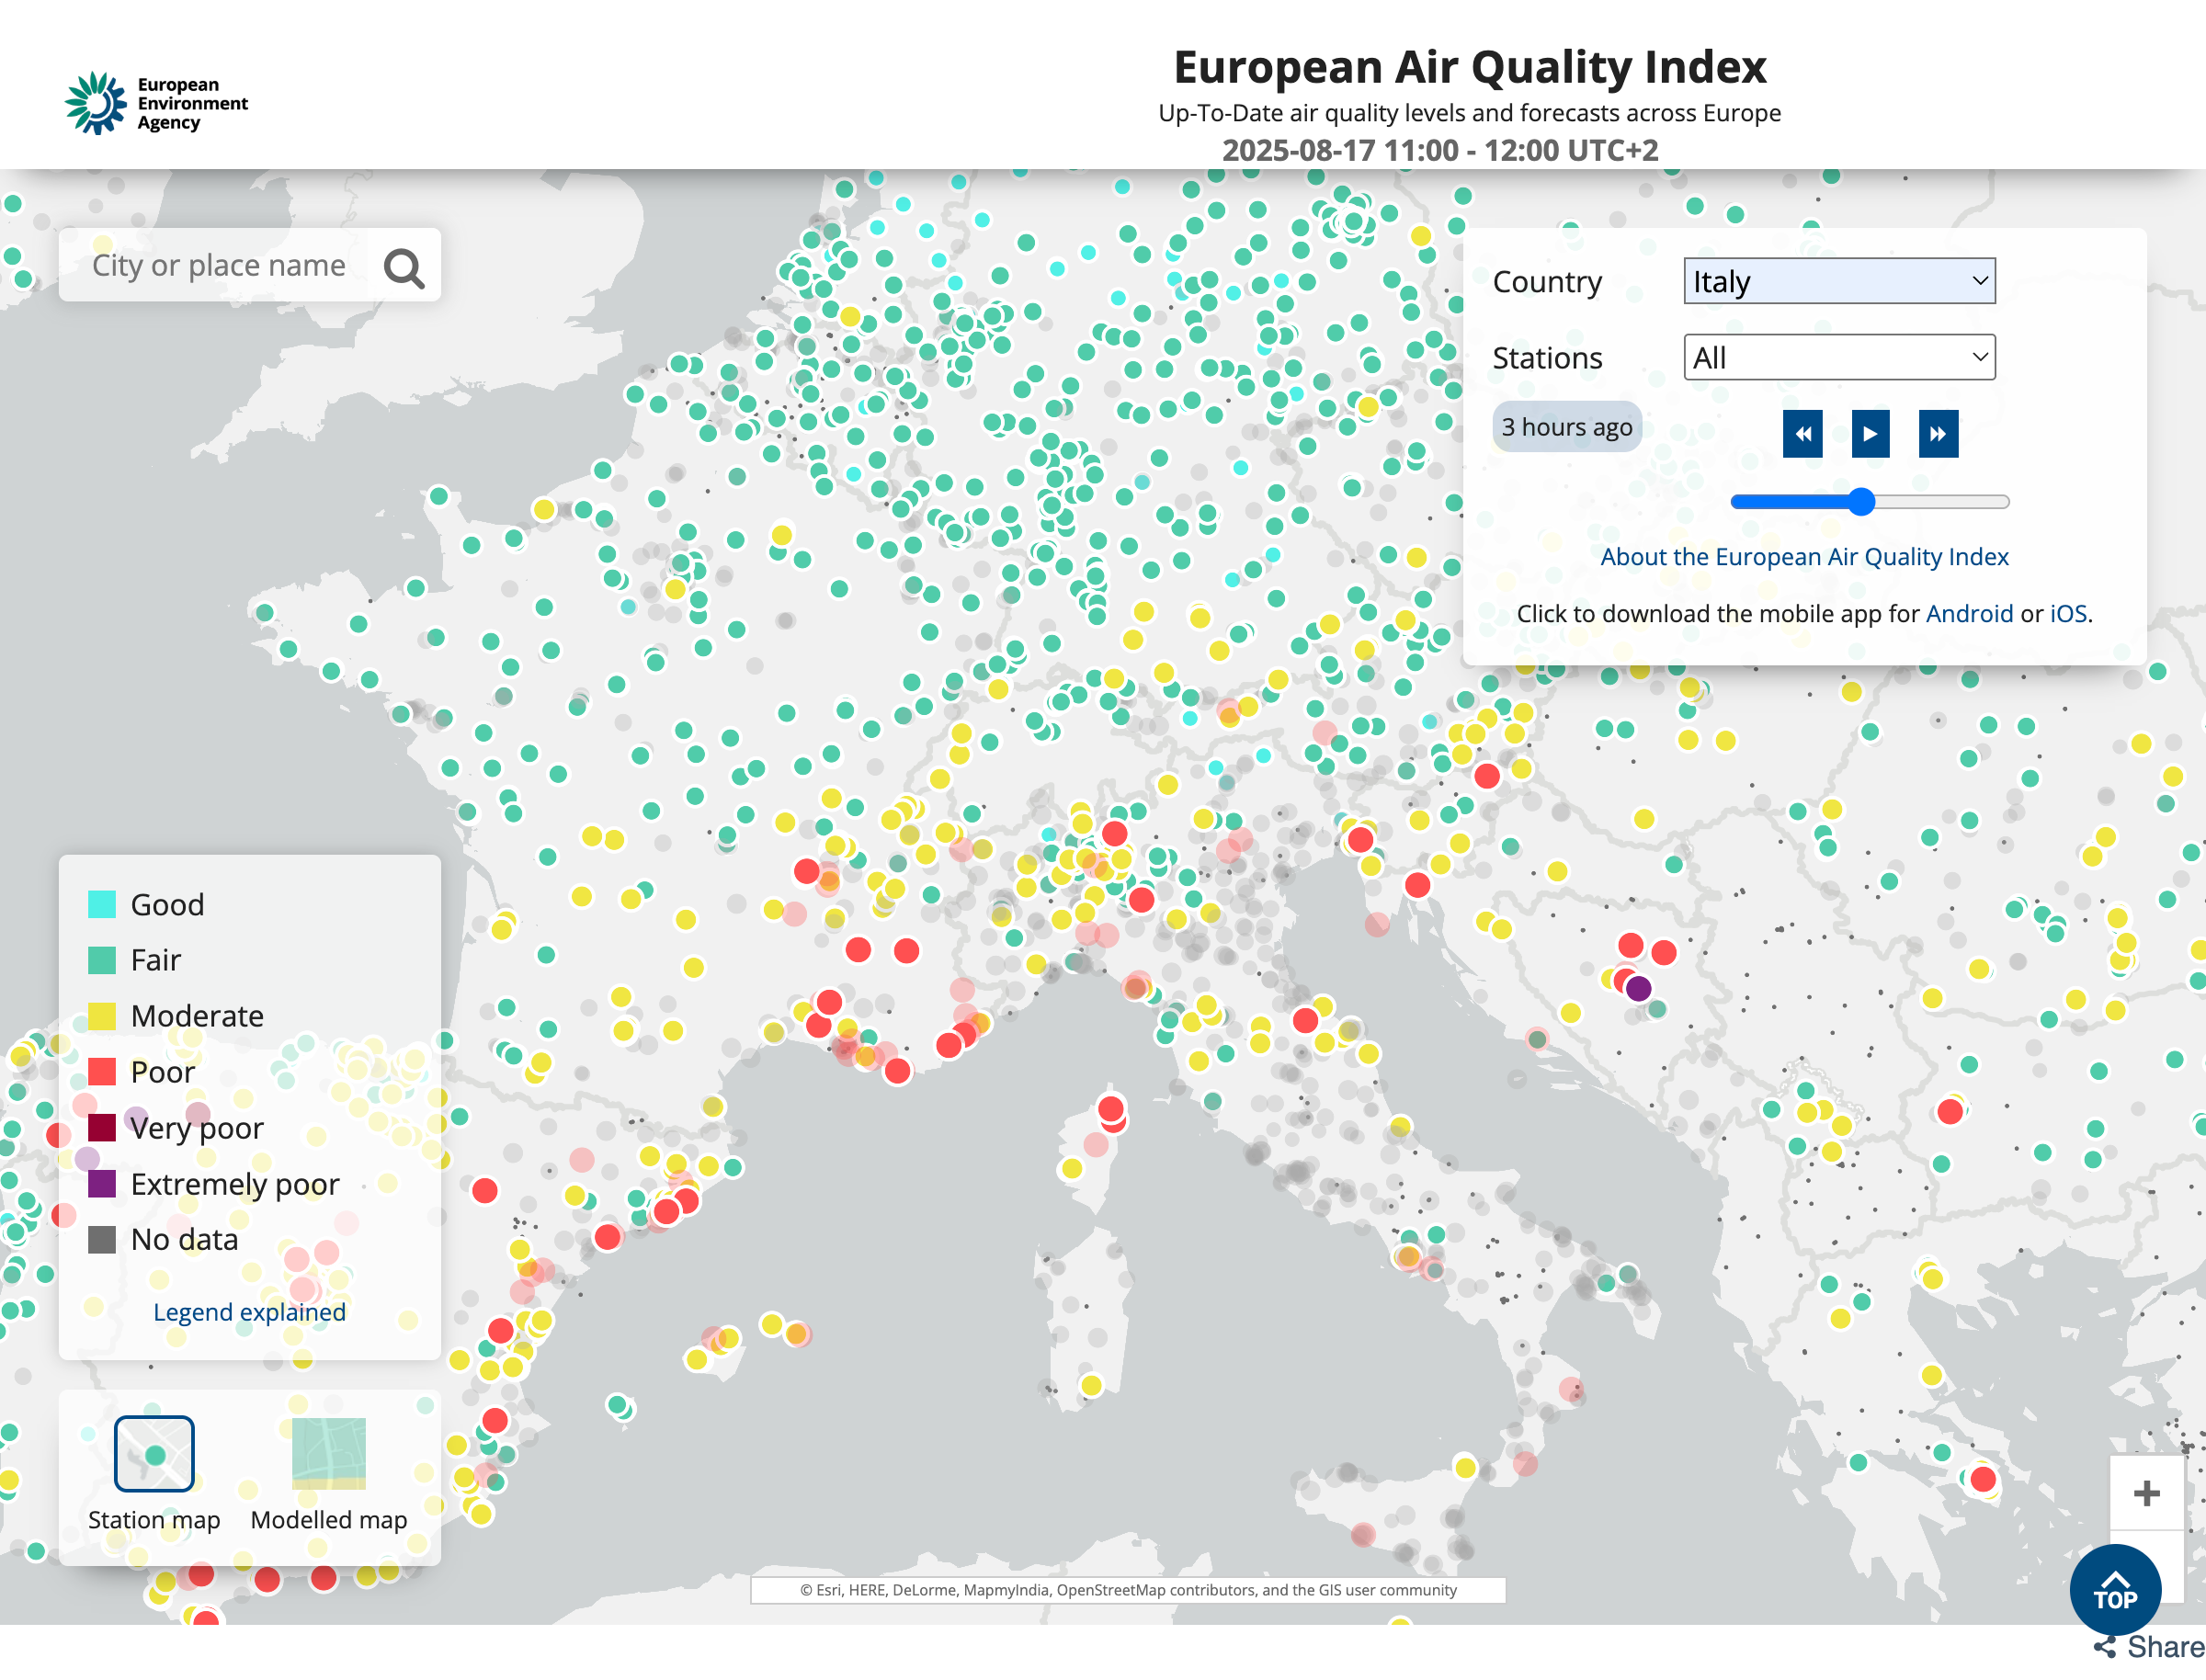
\includegraphics[width=\textwidth]{eaqi3.png}
  \caption{European Air Quality Index per Bologna: (sopra) Mappa "modellata" interattiva, (sotto) Mappa "a stazioni" interattiva}
  \label{fig:eaqi-combined}
\end{figure}
\section{Principali inquinanti atmosferici e loro origini}

La valutazione della qualità dell'aria si basa sul monitoraggio di specifici contaminanti presenti nell'atmosfera.
Secondo \citet{GoogleMapsAirQuality2024}, i parametri più frequentemente rilevati nelle aree urbane includono i seguenti elementi.

\subsection{Materiale particolato (PM)}

Insieme di particelle microscopiche, solide e liquide, sospese nell'atmosfera.
Le frazioni PM$_{10}$ e PM$_{2.5}$ identificano particelle con diametro rispettivamente inferiore a 10 e 2,5 micrometri.
Le principali sorgenti comprendono:

\begin{itemize}
  \item Traffico veicolare e combustione nei motori
  \item Riscaldamento domestico a biomassa
  \item Processi industriali
  \item Fenomeni naturali come incendi boschivi e tempeste di sabbia
\end{itemize}

\subsection{Biossido di azoto NO2}

Gas caratteristico dell'inquinamento urbano, generato prevalentemente da:

\begin{itemize}
  \item Emissioni del trasporto su strada
  \item Attività industriali
  \item Impianti di produzione energetica
  \item Sistemi di riscaldamento civile
\end{itemize}

\subsection{Ozono troposferico O3}

Diversamente dall'ozono stratosferico che ci protegge dai raggi UV, quello presente negli strati bassi dell'atmosfera
costituisce un inquinante secondario. Si forma attraverso reazioni fotochimiche tra:

\begin{itemize}
  \item Composti organici volatili
  \item Ossidi di azoto
  \item Radiazione solare
\end{itemize}

Le fonti primarie dei precursori sono veicoli, centrali termoelettriche e processi industriali.

\subsection{Anidride solforosa SO2}

Gas dall'odore caratteristico e dalle proprietà irritanti, originato da:

\begin{itemize}
  \item Combustione di carbone e derivati petroliferi negli impianti energetici
  \item Raffinazione del petrolio
  \item Produzione di cemento
  \item Attività vulcanica
\end{itemize}

\subsection{Monossido di carbonio (CO)}

Gas inodore e tossico prodotto dalla combustione incompleta di combustibili fossili in veicoli e macchinari industriali.

\section{Sistema di coordinate}

Nella sezione seguente verranno introdotti i sistemi di coordinate presenti nei sistemi di elaborazione trattati.

\subsection{EPSG:4326}

Per il progetto di tesi, sono state utilizzate come base per la collocazione dei sensori di rilevamento della qualità dell'aria le mappe di OpenStreetMap. Tale strumento utilizza il sistema di coordinate WGS84 (World Geodetic System 1984) per rappresentare latitudine e longitudine.

Nello specifico, il sistema di riferimento prevede un formato di coordinate geografiche decimali, in codice EPSG 4326. L'acronimo EPSG sta per European Petroleum Survey Group, fondato negli anni '80 dall'industria petrolifera europea con scopo originale la standardizzazione dei sistemi di coordinate per l'esplorazione petrolifera offshore nel Mare del Nord. Le compagnie petrolifere infatti usavano sistemi di coordinate diversi, creando confusione e errori costosi \cite{iogp2019, ashkenazi1984}.

Dal 1986 al 2005, tale sistema di coordinate viene gestito dall'European Petroleum Survey Group. Dal 2005 ad oggi, viene trasferito alla International Association of Oil \& Gas Producers (IOGP), ma il nome EPSG è rimasto di comune utilizzo.

Il registro EPSG è diventato lo standard mondiale per i sistemi di coordinate (Coordinate Reference Systems - CRS), i datum geodetici, le proiezioni cartografiche, le trasformazioni tra sistemi e le unità di misura.

Andiamo a definire ciascuno degli elementi elencati:

\begin{itemize}
\item Sistemi di coordinate (CRS): Un framework completo che definisce come identificare univocamente ogni punto sulla Terra usando numeri, come latitudine/longitudine o coordinate piane.
\item Datum geodetici: la forma matematica di riferimento della Terra (ellissoide) e il suo posizionamento nello spazio, che serve come ``punto zero'' per tutte le misurazioni.
\item Proiezioni cartografiche: i metodi matematici per ``appiattire'' la superficie curva della Terra su una mappa bidimensionale.
\item Trasformazioni tra sistemi: le formule matematiche per convertire coordinate da un sistema di riferimento a un altro.
\item Unità di misura: le scale di riferimento per esprimere distanze, angoli e posizioni (metri, gradi, piedi, radianti, ecc.) all'interno di ciascun sistema di coordinate.
\end{itemize}

Ogni sistema di coordinate ha un codice EPSG univoco:

\begin{itemize}
\item EPSG:4326 = WGS84 (lat/lon in gradi) \cite{epsg4326}.
\item EPSG:3857 = Web Mercator (usato da Google Maps) \cite{epsg3857}.
\item EPSG:32633 = UTM zone 33N (comune in Italia centrale) \cite{epsg32633}.
\item EPSG:3003 = sistema italiano storico. Italy zone 1 \cite{epsg3003}.
\end{itemize}

Il sistema utilizzato per il progetto è il datum WGS84, codice EPSG:4326, in formato di coordinate geografiche decimali che rappresenta la latitudine, la longitudine, con una precisione fino a 7-8 cifre decimali.

Il riferimento fondamentale per il calcolo della latitudine è l'Equatore (latitudine 0°), definito come il cerchio massimo che divide la Terra in emisfero Nord e Sud. Si misura come angolo dal piano equatoriale verso nord o sud con un range da -90° (Polo Sud) a +90° (Polo Nord). I paralleli di riferimento sono:

\begin{itemize}
\item Tropico del Cancro: 23°27'N
\item Tropico del Capricorno: 23°27'S
\item Circolo Polare Artico: 66°33'N
\item Circolo Polare Antartico: 66°33'S
\end{itemize}

Di seguito un'immagine rappresentativa \ref{fig:paralleli-della-terra}.

\begin{figure}[H]
  \centering
  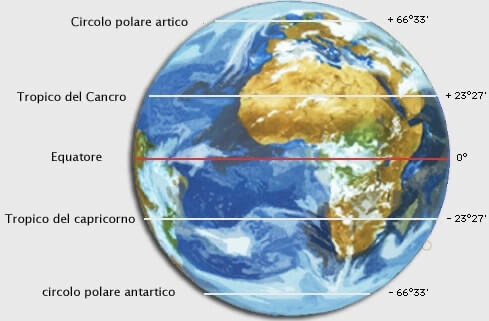
\includegraphics[width=\textwidth]{paralleli-della-terra.png}
  \caption{Paralleli della terra \cite{chimica-online-equatore}.}
  \label{fig:paralleli-della-terra}
\end{figure}

Per la longitudine, il riferimento principale è il Meridiano di Greenwich (longitudine 0°), definito come il meridiano che passa per l'Osservatorio Reale di Greenwich, London. È stato stabilito nel 1884 alla Conferenza Internazionale del Meridiano, e si misura come angolo dal meridiano di Greenwich verso est o ovest con un range da -180° (ovest) a +180° (est). I meridiani di riferimento sono:

\begin{itemize}
\item Linea del Cambio di Data: 180°
\item Antimeridiano: Opposto a Greenwich
\end{itemize}

Il sistema di coordinate geografiche funziona come una griglia sferica, dove la latitudine sono le linee orizzontali (paralleli), la longitudine sono le linee verticali (meridiani), e le unità sono espresse in gradi decimali o gradi-minuti-secondi.

Anche se OSM memorizza i dati in WGS84, per la visualizzazione delle mappe utilizza spesso la proiezione Web Mercator (EPSG:3857), che è quella usata anche da Google Maps, Bing Maps e altri servizi di mappe online. Questa proiezione ``schiaccia'' le aree polari ma mantiene gli angoli, rendendola ideale per la navigazione. La proiezione Web Mercator (nota anche come Pseudo-Mercator o Google Mercator) è la proiezione cartografica più utilizzata per le mappe online moderne.

\subsection{EPSG:3857}

La proiezione WebMercator con codice EPSG:3857 (o EPSG:900913), rappresenta la terra come una sfera perfetta, invece che come un ellissoide rappresentato dallo standard WGS84. Utilizza come unità i metri.

La proiezione ``avvolge'' la Terra con un cilindro tangente all'equatore, poi proietta tutti i punti sulla superficie del cilindro. Tale sistema ha come vantaggio la conservazione degli angoli, la facilità di implementazione nei sistemi informatici, uno zoom semplice da utilizzare e un tile system efficiente che divide la mappa in quadrati per il caricamento veloce.

Gli svantaggi tuttavia sono la distorsione sia delle aree che delle distanze: infatti la Groenlandia appare grande quanto l'Africa, ma in realtà l'Africa è 14 volte più grande. Le distanze soprattutto alle latitudini elevate appaiono estremamente distorte. Inoltre non vengono mostrati i poli: la proiezione si interrompe infatti a circa 85°N e 85°S.

Rimane comunque il sistema più diffuso tra i servizi di mappe online, quali Google Maps, OpenStreetMap, Bing Maps, Apple Maps, Mapbox. Infatti risulta molto efficiente per la navigazione urbana e la consultazione online, ma di scarso valore per analisi geografiche che richiedono precisione nelle aree o distanze.

\subsection{WGS84}

Il sistema WGS84 fu creato dal Dipartimento della Difesa USA negli anni '80, ufficializzato nel 1984, rivisto nel 1996 e 2004, e periodicamente raffinato. Lo scopo originale era creare un sistema unificato per il GPS militare americano \cite{wgs84updates}.

WGS84 definisce la forma della Terra usando un ellissoide di riferimento con questi parametri che definiscono il modello matematico della Terra, la quale nella realtà è un geoide.

\paragraph{Semiasse maggiore ($a$)} è il raggio equatoriale della Terra, definito come distanza dal centro della Terra all'equatore. Il valore è di 6.378.137 m.

\paragraph{Schiacciamento ($f$)} misura quanto la Terra è ``schiacciata'' ai poli. Tale valore risulta in uno schiacciamento della Terra del 0,34\%, in quanto la Terra non è una sfera perfetta. Il valore numerico è di ${298{,}257223563}^{-1}$.

Formula: 
\begin{equation}
f = \frac{a - b}{a}
\end{equation}

\paragraph{Semiasse minore ($b$)} è il raggio polare della Terra, definito come distanza dal centro della Terra ai poli. Risulta circa 21,4 km più corto del semiasse maggiore, con un valore di 6.356.752,314245 metri.

Formula: 
\begin{equation}
b = a \times (1 - f)
\end{equation}

\paragraph{Eccentricità} misura la deviazione dalla forma sferica. Per un valore vicino a 0, si ha una sfera perfetta. Il valore WGS84 indica un ellissoide molto vicino alla sfera.

Eccentricità = 0,0818191908

Formula: 
\begin{equation}
e^2 = \frac{a^2 - b^2}{a^2}
\end{equation}

Il sistema di coordinate 3D ha origine nel centro di massa terrestre, con un sistema di riferimento temporale basato sul Tempo Atomico Internazionale. Possiede una precisione teorica centimetrica, mentre l'accuratezza pratica dipende dal metodo di misurazione.

Di seguito il modello dell'elissoide WGS84 \ref{fig:elissoide-wgs84}.

\begin{figure}[H]
  \centering
  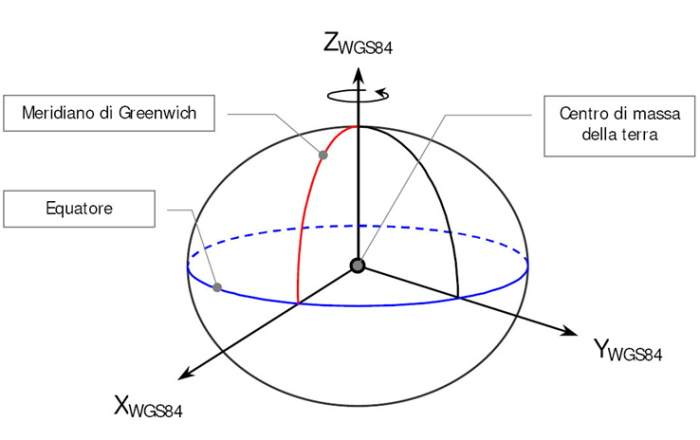
\includegraphics[width=\textwidth]{Sistema_WGS84.png}
  \caption{Ellissoide WGS84 \cite{topgeometri}.}
  \label{fig:elissoide-wgs84}
\end{figure}

\section{OpenStreetMap}

OpenStreetMap (OSM) è un progetto collaborativo di mappatura web che raccoglie dati geospaziali per creare e distribuire mappe online, liberamente disponibili a chiunque abbia una connessione Internet \cite{neis2012}. Una volta accessibile, OpenStreetMap (OSM) permette agli utenti Internet di contribuire e modificare i dati geospaziali, rendendolo di fatto l'equivalente cartografico di Wikipedia.

OpenStreetMap (OSM) è emerso come un progetto globale e una comunità che opera con l'obiettivo di creare e mantenere un database libero e modificabile e una mappa del mondo basata sui contributi di volontari cartografi \cite{fonte2022}. Con il suo database che include quasi 7,5 miliardi di punti dati (nodi), contribuiti da circa 1,8 milioni di utenti a marzo 2022, è forse l'esempio più riuscito di un progetto di geoinformazione crowdsourced e del concetto di informazione geografica volontaria \cite{fonte2022}.

\subsection{Storia e fondazione}

Il progetto OpenStreetMap (OSM) è stato fondato nel 2004 nel Regno Unito da Steve Coast, allora studente presso l'University College London \cite{osmhistory2024}, il quale ne ha registrato il dominio \href{openstreetmap.org}{openstreetmap.org} \cite{osmhistory2024}. La prima strada è stata inserita il 10 dicembre 2004 dopo che Steve aveva pedalato intorno a Regent's Park a Londra con un ricevitore GPS \cite{coast2004}.

Il 22 agosto 2006, la OpenStreetMap Foundation è stata istituita per incoraggiare la crescita, lo sviluppo e la distribuzione di dati geospaziali liberi e fornire dati geospaziali per chiunque li usi e li condivida \cite{osmfoundation2006}.

\subsection{Caratteristiche tecniche}

OpenStreetMap (OSM) è mantenuto da cartografi volontari di tutto il mondo che utilizzano dispositivi GPS, fotocamere portatili e laptop per la mappatura sul campo. I dati raccolti sono integrati con fotografie aeree open source digitalizzate e mappe gratuite da fonti governative e commerciali \cite{neis2012}.

Il progetto utilizza il sistema di coordinate WGS84 (EPSG:4326) per rappresentare latitudine e longitudine, permettendo l'integrazione con sistemi GPS e altre piattaforme cartografiche digitali.

OSM è stato definito come ``la wikificazione delle mappe'' da alcuni ricercatori \cite{sehra2013}, evidenziando il parallelo con il modello collaborativo di Wikipedia. Il progetto ha attirato considerevole attenzione da molteplici attori, incluse industrie, governi e organizzazioni umanitarie \cite{fonte2022}.

\subsection{Applicazioni e ricerca accademica}

La comunità accademica ha mostrato un interesse duraturo per OSM, documentato in diverse recenti review \cite{vargas2020, sehra2013}. Le applicazioni di ricerca includono studi sulla qualità dei dati, analisi delle dinamiche della comunità OSM, e utilizzo dei dati OSM per applicazioni di machine learning e remote sensing \cite{vargas2020}.

OpenStreetMap (OSM) rappresenta oggi uno dei più grandi progetti di dati aperti su Internet e un esempio notevole di sistemi di informazione geografica partecipativa (participatory GIS) \cite{quinn2022}.

\subsection{Struttura dati di OpenStreetMap (OSM)}

Per rappresentare informazioni geografiche, OpenStreetMap (OSM) utilizza un modello dati basato su tre elementi fondamentali: nodi (\textit{nodes}), percorsi (\textit{ways}) e relazioni (\textit{relations}) \cite{elements2024}.

\paragraph{Nodi (\textit{Nodes})}

Un nodo rappresenta un singolo punto geografico sulla mappa, caratterizzato da:
\begin{itemize}
\item Un identificatore numerico unico a 64 bit
\item Coordinate geografiche (latitudine e longitudine) in WGS84
\item Un set opzionale di tag (coppie chiave-valore)
\item Numero di versione e timestamp per il controllo delle modifiche
\end{itemize}

I nodi possono rappresentare elementi puntuali come punti di interesse (negozi, semafori, fermate autobus \dots) oppure essere utilizzati come vertici per definire la geometria di percorsi più complessi \cite{osmdata2024}.

\paragraph{Percorsi (\textit{Ways})}
Un percorso è una sequenza ordinata di nodi che forma una polilinea o un poligono chiuso. I percorsi non memorizzano direttamente la loro posizione geografica, ma mantengono una lista ordinata di identificatori di nodi \cite{osmdata2024}. Possono rappresentare:
\begin{itemize}
\item Elementi lineari: strade, fiumi, confini
\item Elementi areali: edifici, laghi, parchi (quando il percorso è chiuso)
\end{itemize}

\paragraph{Relazioni (\textit{Relations})}
Le relazioni sono collezioni strutturate di oggetti (nodi, percorsi o altre relazioni) utilizzate per definire relazioni logiche o geografiche tra elementi diversi \cite{relations2024}. Ogni membro di una relazione può avere un ruolo opzionale che descrive la sua funzione. Esempi includono:
\begin{itemize}
\item Multipoligoni (aree con buchi o confini complessi)
\item Percorsi di trasporto pubblico
\item Confini amministrativi
\item Limitazioni di svolta
\end{itemize}

\paragraph{Sistema di tag}
Tutti gli elementi OSM possono essere descritti attraverso tag, costituiti da coppie chiave-valore in formato Unicode (massimo 255 caratteri) \cite{mapfeatures2024}. Il sistema di tagging libero permette di includere un numero illimitato di attributi per ogni elemento, con la comunità che si accorda su combinazioni standard per le caratteristiche più comuni.

\subsection{Applicazioni e casi d'uso}

OpenStreetMap (OSM) trova applicazione in numerosi contesti, dalla ricerca accademica alle applicazioni commerciali e umanitarie.

\paragraph{Ricerca accademica}
OSM rappresenta una risorsa preziosa per la ricerca in diversi ambiti:
\begin{itemize}
\item \textbf{Machine Learning e Remote Sensing}: utilizzato per training di modelli di classificazione del territorio e miglioramento della copertura dei dati \cite{vargas2020}.
\item \textbf{Analisi urbana}: studio della qualità dell'aria, accessibilità, pianificazione dei trasporti.
\item \textbf{Analisi della mobilità}: creazione di database nazionali per infrastrutture ciclabili \cite{sfu2022}.
\end{itemize}

\paragraph{Applicazioni commerciali}
Molte aziende utilizzano OSM come base per i loro servizi:
\begin{itemize}
\item Servizi di mappe (Facebook, Foursquare, Strava).
\item Applicazioni di delivery e logistica.
\item Servizi di car sharing e bike sharing.
\item Piattaforme di e-commerce per localizzazione servizi.
\end{itemize}

\subsection{Integrazione programmatica}

Per integrare i dati OSM in applicazioni software, sono disponibili diverse librerie e strumenti.

\paragraph{API e strumenti di accesso ai dati}

OpenStreetMap (OSM) fornisce diversi metodi per accedere e interrogare i suoi dati, adatti a diverse esigenze applicative.

\paragraph{Overpass API}
L'Overpass API è un motore di database ottimizzato per interrogazioni di sola lettura sui dati OSM \cite{overpass2024}. A differenza dell'API principale ottimizzata per l'editing, Overpass API è progettata per consumatori di dati che necessitano di pochi elementi selezionati rapidamente o fino a circa 10 milioni di elementi in alcuni minuti, utilizzando criteri di ricerca come posizione, tipo di oggetti, proprietà dei tag o combinazioni di questi \cite{overpass2024}.

L'API utilizza un linguaggio di query specializzato (Overpass QL) e offre diversi formati di output tra cui XML, JSON, e CSV. Le query possono essere testate interattivamente attraverso Overpass Turbo \cite{overpassturbo2024}, un'interfaccia web che permette di visualizzare i risultati su una mappa interattiva.

Ad esempio, per la scelta della collocazione dei sensori, è stata realizzata una query per ottenere tutti gli incroci fra le arterie principali e le strade secondarie del comune di Bologna. Questa scelta è stata fatta in quanto tali intersezioni, soprattutto quelle semaforizzate, costituiscono zone di concentrazione delle emissioni veicolari, dove il traffico in attesa genera un incremento localizzato dell'inquinamento atmosferico, rendendo quindi la misurazione più significativa.

La seguente query \ref{lst:esempio} in Overpass QL estrae tali intersezioni:

\begin{lstlisting}[caption={Query Overlpass QL di esempio}, label=lst:esempio]
[out:json][timeout:90];

// Area corrispondente al comune di Bologna 
area[name="Bologna"][admin_level=8]->.bologna;

// Strade principali
(
  way(area.bologna)["highway"="motorway"];
  way(area.bologna)["highway"="trunk"];
  way(area.bologna)["highway"="primary"];
  way(area.bologna)["highway"="secondary"];
  way(area.bologna)["highway"="tertiary"];
)->.major;

// Strade secondarie
(
  way(area.bologna)[highway="unclassified"];
  way(area.bologna)[highway="residential"];
  way(area.bologna)[highway="living_street"];
  way(area.bologna)[highway="service"];
  way(area.bologna)[highway="pedestrian"];
  way(area.bologna)[highway="track"];
)->.minor;

// Intersezioni stradali
node(w.major)(w.minor);
out;
\end{lstlisting}

\begin{figure}[H]
  \centering
  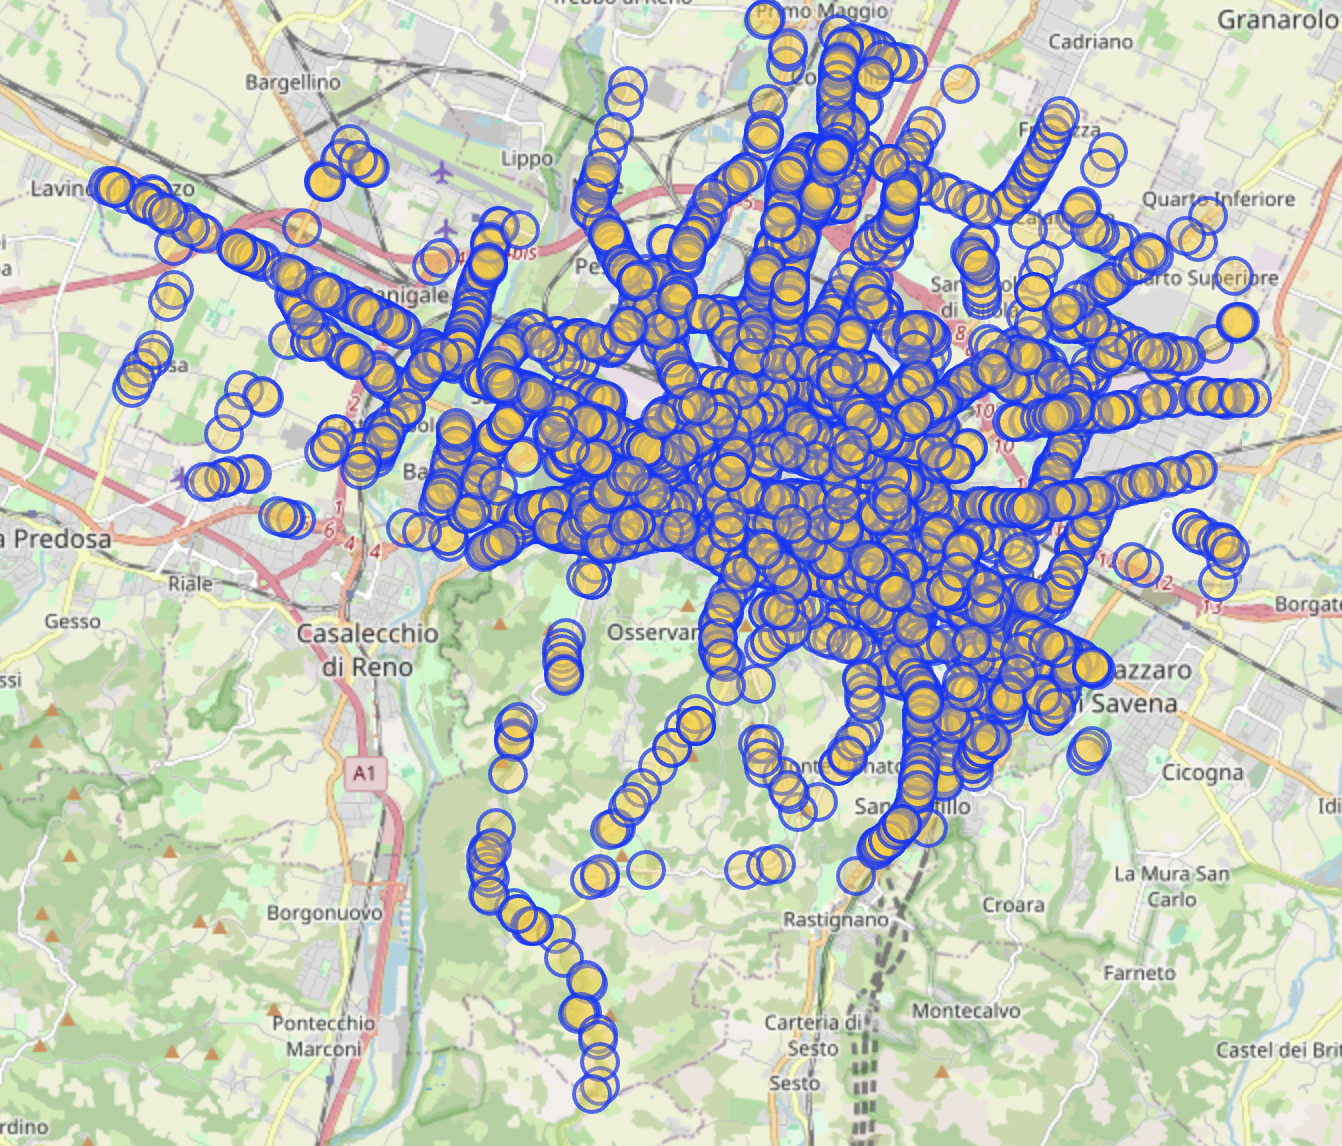
\includegraphics[width=\textwidth]{major_minor_streets_intersection.png}
  \caption{Intersezioni fra le strade principali e secondarie nel comune bolognese}
  \label{fig:streets-intersections}
\end{figure}

\paragraph{Formati di dati}
I dati OSM sono disponibili in diversi formati \cite{geoapify2024}:
\begin{itemize}
\item \textbf{OSM XML}: formato nativo basato su XML
\item \textbf{PBF}: formato binario compresso per maggiore efficienza
\item \textbf{GeoJSON}: per integrazione con applicazioni web
\item \textbf{Shapefile}: per compatibilità con software GIS tradizionali
\end{itemize}

L'ecosistema di strumenti e API di OpenStreetMap (OSM) offre quindi una piattaforma completa e flessibile per lo sviluppo di applicazioni geospaziali, dalla semplice visualizzazione di mappe fino a complessi sistemi di analisi territoriale e routing.

\section{Funzionalità del sistema}

La presente sezione illustra in modo approfondito i requisiti del sistema da implementare, derivanti dallo studio preliminare.
Il progetto di tesi si propone di sviluppare un'applicazione web conforme ai requisiti funzionali e non funzionali che verranno esposti.

\subsection{Requisiti funzionali}

\begin{itemize}
    \item Visualizzazione della mappa: l'utente dovrà poter visualizzare una mappa in cui
    \begin{itemize}
        \item verrà centrata l'area interessata dall'applicativo
        \item verranno mostrate le misurazioni in tempo reale ed i conseguenti AQI relativi ai sensori
        \item sarà possibile scegliere quali livelli osservare
        \item sarà presentato un livello heatmap le AQI ed ogni altro inquinante in esame
        \item sarà possibile arrestare e riprendere la raccolta delle registrazioni live
        \item verranno predisposte tabelle per elencare sensori, misurazioni, statistiche e log
        \item dovrà essere possibile visualizzare le informazioni relative ad ogni sensore quali nome, posizione, data ultima registrazione, livello di qualità dell'aria corrente e livelli singoli inquinanti
    \end{itemize}
    \item Fruizione dei dati: verranno predisposte delle rotte specifiche per fare interrogazioni preformate alle registrazioni salvate.
\end{itemize}

\subsection{Requisiti non funzionali}

\begin{itemize}
    \item Design: l'interfaccia web dovrà essere mobile-first nativamente e responsive.
    \item Usabilità: l'interfaccia web dovrà risultare semplice ed intuitiva, rendendo l'esperienza più semplice, favorendo elementi grafici come colori e simboli rispetto al testo.
    \item Deployment: il progetto dev'essere strutturato in modo da essere eseguito in un ambiente virtualizzato, rendendo così il deploy possibile attraverso un solo comando. L'installazione di dipendenze deve limitarsi esclusivamente agli strumenti di containerizzazione e/o virtualizzazione appropriati.
\end{itemize}

\section{Principali difficoltà del progetto}

Le principali sfide affrontate durante lo sviluppo del progetto riguardano:

\begin{itemize}
    \item La gestione delle misurazioni registrate e l'orchestrazione dei vari microservizi.
    \item La generazione di pseudo misurazioni aleatorie (mocking).
    \item La visualizzazione in tempo reale dei dati sulla mappa e la corretta presentazione della heatmap (mappa di calore) dei correnti AQI relativi ai rispettivi sensori.
\end{itemize}